\documentclass{article}
\usepackage{hyperref}
\usepackage{pdfpages}
\usepackage{tikz}
\usepackage{float}
\usetikzlibrary{matrix, shapes, chains, shapes.geometric, arrows, positioning}
\tikzstyle{startstop} = [rectangle, rounded corners, minimum width=3cm, minimum height=1cm,text centered, draw=black, fill=red!30]
\tikzstyle{io} = [trapezium, trapezium left angle=70, trapezium right angle=110, minimum width=3cm, minimum height=1cm, text centered, draw=black, fill=blue!30]
\tikzstyle{process} = [rectangle, minimum width=3cm, minimum height=1cm, text centered, draw=black, fill=orange!30]
\tikzstyle{decision} = [diamond, minimum width=3cm, minimum height=1cm, text centered, draw=black, fill=green!30]
\tikzstyle{arrow} = [thick,->,>=stealth]
\tikzset{
    desicion/.style={
        diamond,
        draw,
        text width=3em,
        text badly centered,
        inner sep=0pt
    },
    block/.style={
        rectangle,
        draw,
        text width=10em,
        text centered,
        rounded corners
    },
    cloud/.style={
        draw,
        ellipse,
        minimum height=2em
    },
    descr/.style={
        fill=white,
        inner sep=2.5pt
    },
    connector/.style={
     -latex,
     font=\scriptsize
    },
    rectangle connector/.style={
        connector,
        to path={(\tikztostart) -- ++(#1,0pt) \tikztonodes |- (\tikztotarget) },
        pos=0.5
    },
    rectangle connector/.default=-2cm,
    straight connector/.style={
        connector,
        to path=--(\tikztotarget) \tikztonodes
    }
}
\title{EMISY Project 21 Portable Compass}
\author{Krzysztof Rudnicki, 307585}
\date{\today}
\begin{document}
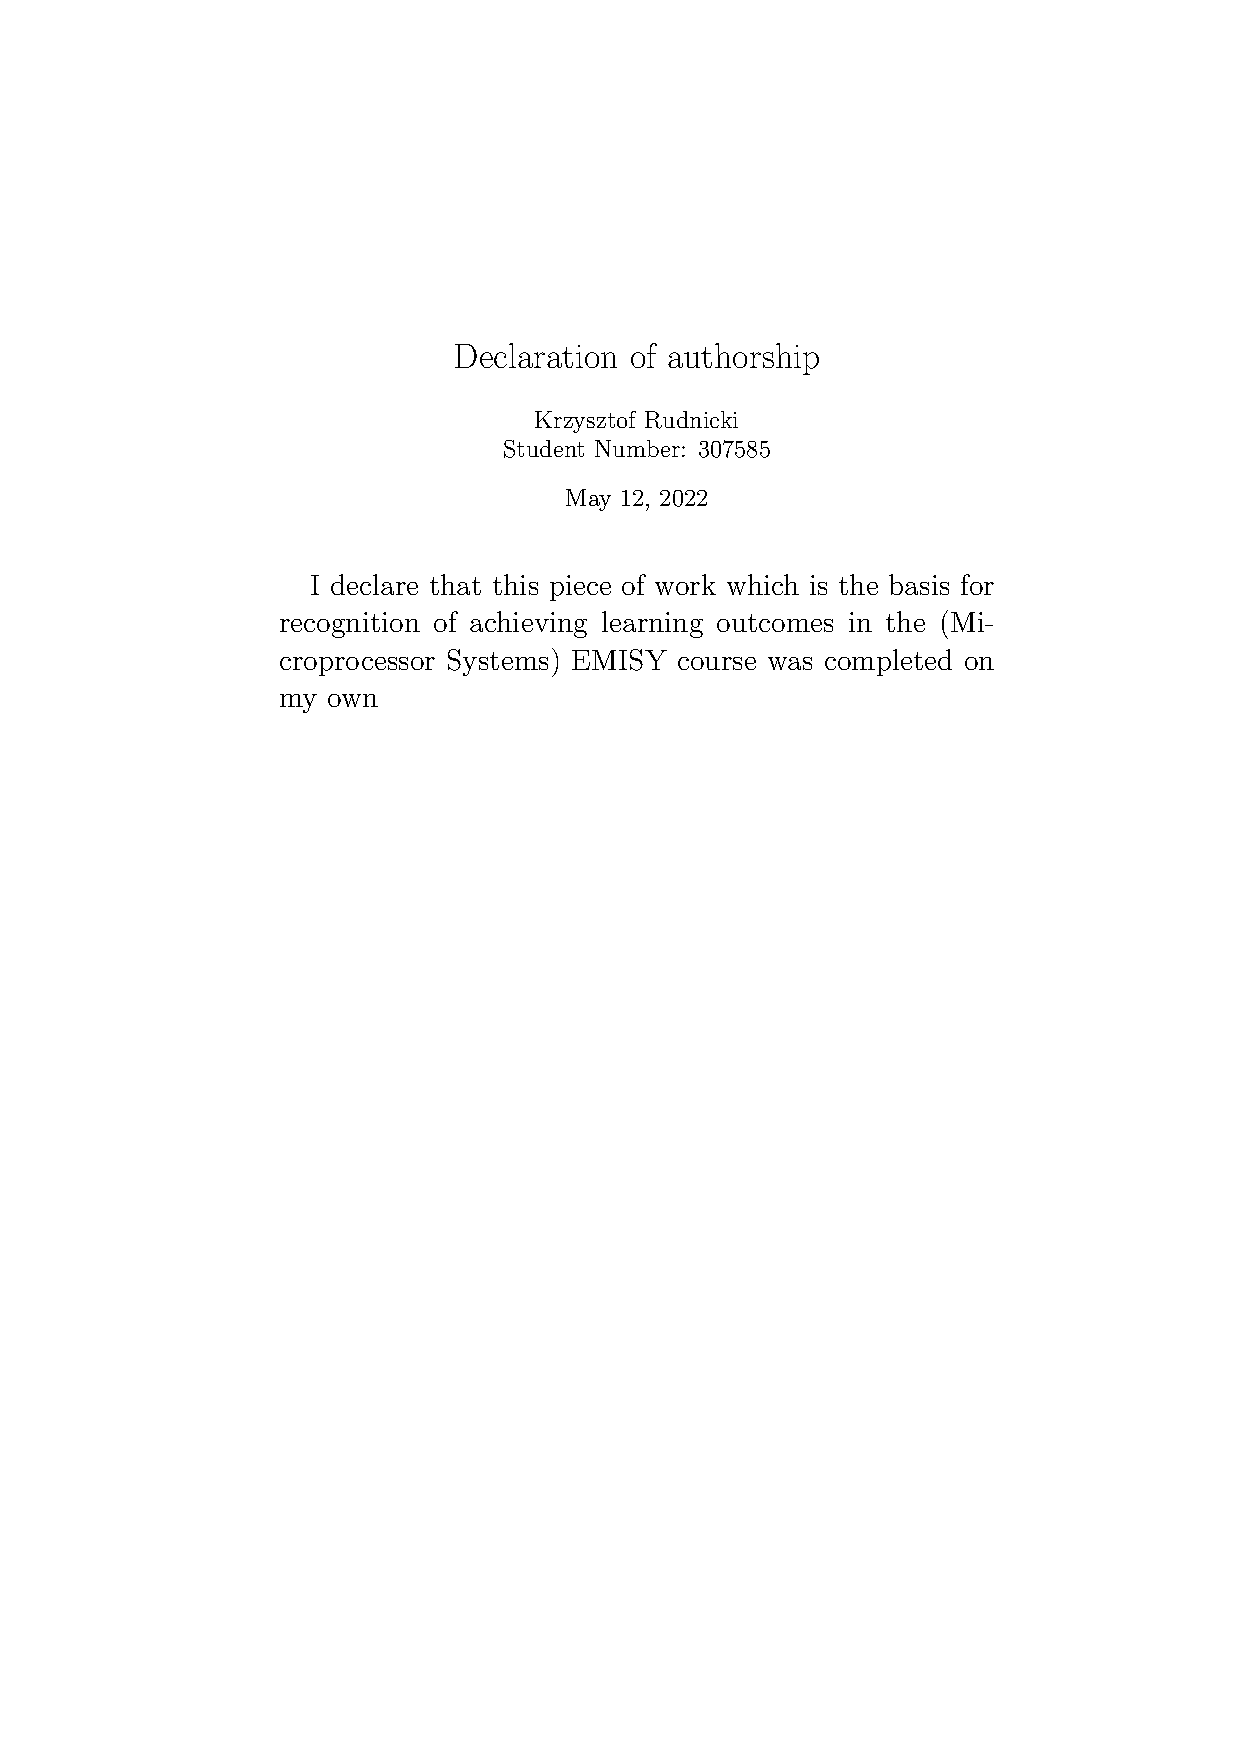
\includepdf[pages={1}]{declaration.pdf}
\maketitle
\section{Analysis of the project}
\subsection{Discussion of project requirements}
We need to create a simple portable compass circuit \\
It should:
\begin{itemize}
	\item Use energy-saving power modes of microcontroller
	\item Be battery powered
	\item Be portable (cellphone/wrist watch)
	\item Communicate using graphical OLED display and two buttons keyboard
\end{itemize}
\subsection{Discussion of solution}
In my solution I focused on picking components based on firstly low power
consumption, then size, then simplicity, whenever I could I tried to do
everything as proposed in the component data sheet. \\
For the schematic itself I needed power saving microcontroller, oled display,
battery, voltage regulator that works well with batteries and digital compass.
\section{Detailed circuit diagram}
\subsection{Diagram itself}
(Diagram is in pdf format so feel free to zoom in if something is not clearly
visible) 
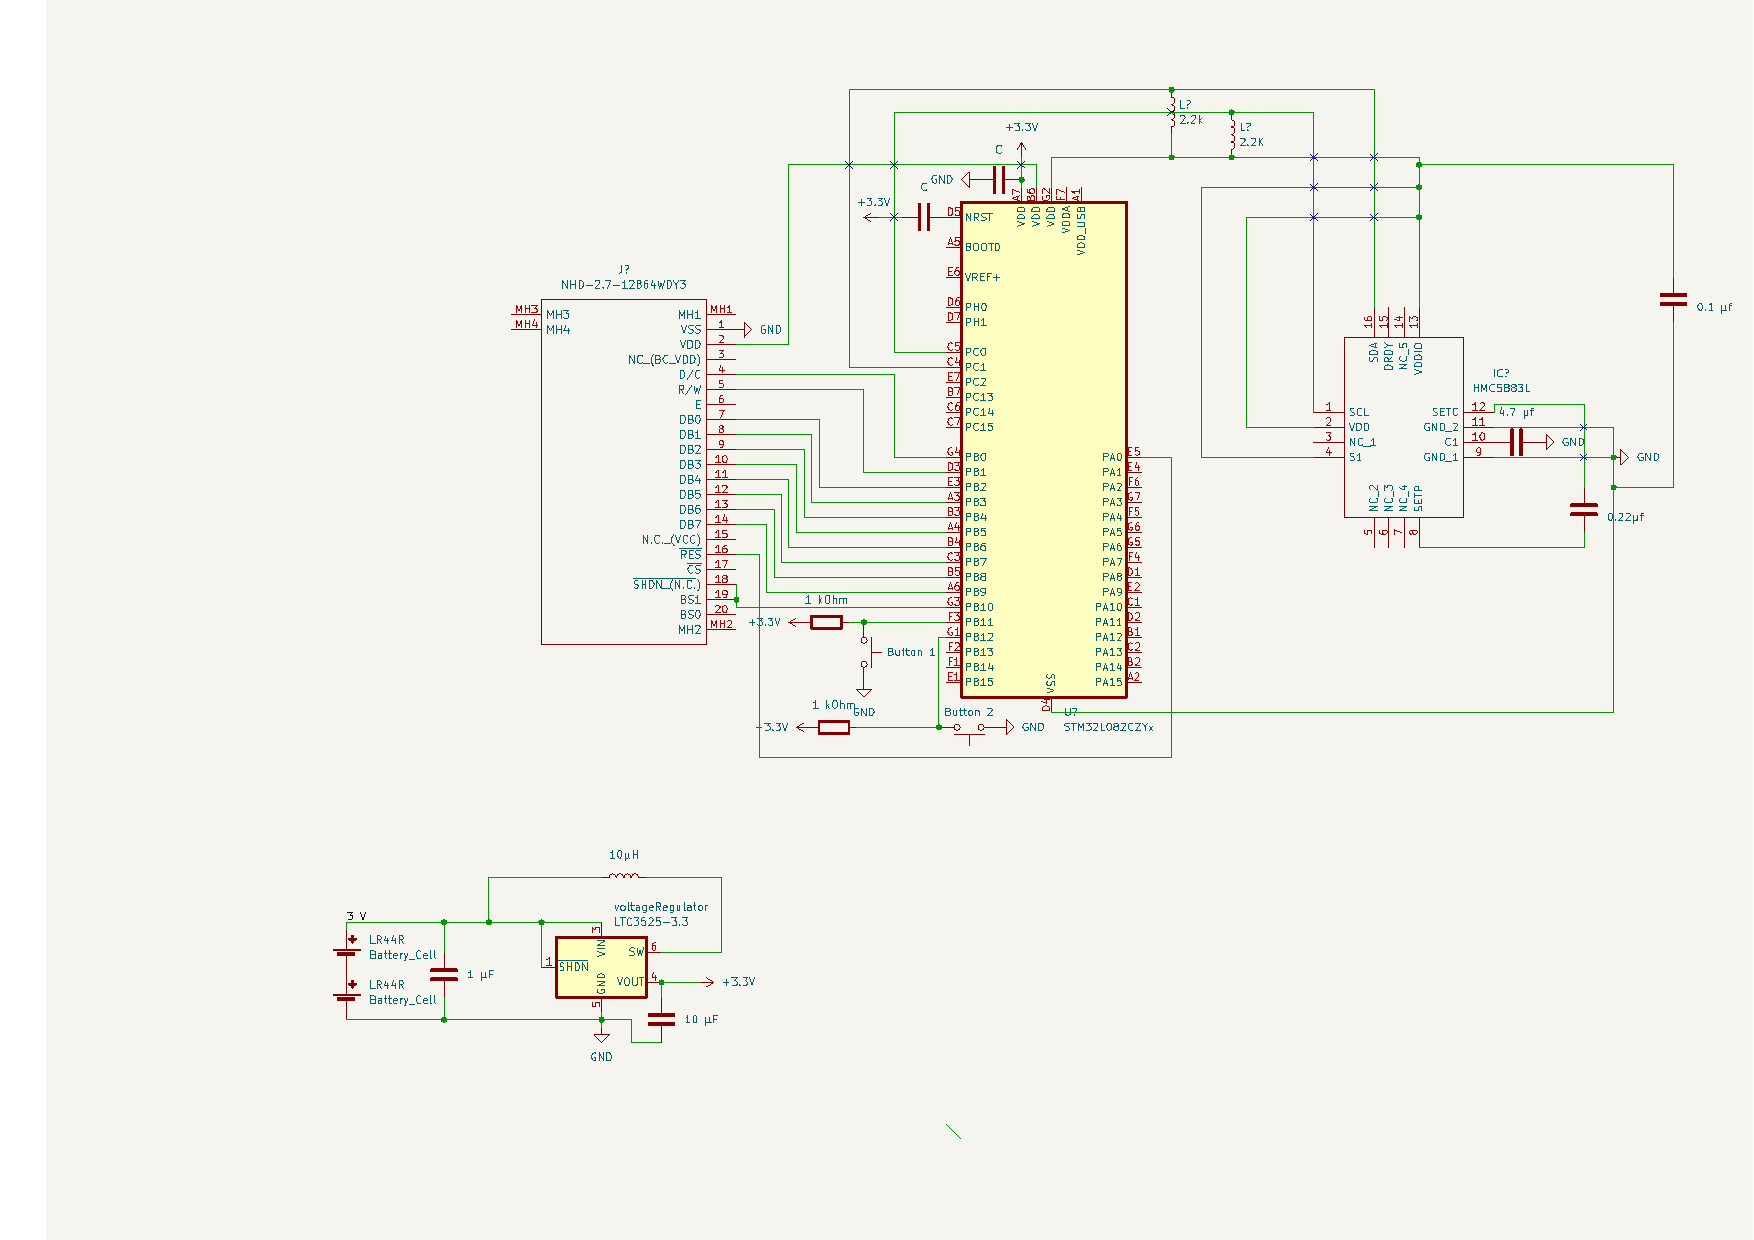
\includepdf[pages=-]{schematicpdf.pdf}
\subsection{Diagram description}
Voltage regulator schematic is done one to one on how it was done in voltage
regulator schematic in case of two battery cells \\ 
Digital compass also was connected exactly as specified in datasheet \\
For OLED I based on the pin descriptions from datasheet and on common patterns
of connecting peripherals \\
Microcontroller itself was pretty straightforward with classic VDD, VSS and
Reset pin conections \\
For buttons I used pull up resistors 
\newpage
\subsection{Components}
\subsubsection{Microcontroller}
I decided to use STM32L082CZ from STM32L0 line
\paragraph{Relatively small} Up to 10 mm $\times$ 10 mm dimensions, 
compared to apple watch display of 34 mm by 40 mm for smaller version. 
\cite{datasheet}
111th page
\paragraph{Square} It is shaped in a square which also simplifies portability
\cite{datasheet} 111th page
\paragraph{Power saving} STM32L0 line was designed specifically for low power
consumption with power consumption as low as 0.29 $\mu$ A in Standby mode
\cite{datasheet} 1st page
\paragraph{Consumer devices} This microcontroller comes from STM32LOx2 line
prepared to be used in consumer devices \cite{consumerDevice}
\paragraph{Ease of use} USB compatible microcontroller and dedicaded debug port
allows for swift code creation.
\cite{datasheet} 1st page 
\subsubsection{All other components}
\paragraph{Oled display} For OLED display I decided to go with
NHD-2.7-12864WDY3. It was an OLED display found on \href{www.mouser.pl}{mouser}
webpage with lowest operating supply current of 180 uA, supply voltage
compatible wit microcontroller (3.3 V) and datasheet not in japanese.
\cite{OLED}
\paragraph{Digital compass} For the compass I used HMC5883L with compatible
voltage, low power consumption of 100 $\mu$ A, compatiblity with battery powered
applications according to datasheet and small size 
\paragraph{Battery} For the battery I choose 2x LR44R series battery, with output
voltage of 1.5 V compatible with voltage regulator (3 V in series), compatible
battery chemistry of Alkaline, 150 mAh capacity for single battery and compact
coin cell shape. \cite{Battery}
\paragraph{Voltage Regulator} For voltage regulator I choose LTC3525-3.3 with high 95 \%
efficiency, desirable output voltage of 3.3 V, low profile and tiny package, it
is also available in kicad by default \cite{Voltage Regulator}
\section{Draft of the microcontroller firmware}
\subsection{Block diagram}
\begin{figure}[H]
	\caption{Start algorithm}
	\centering
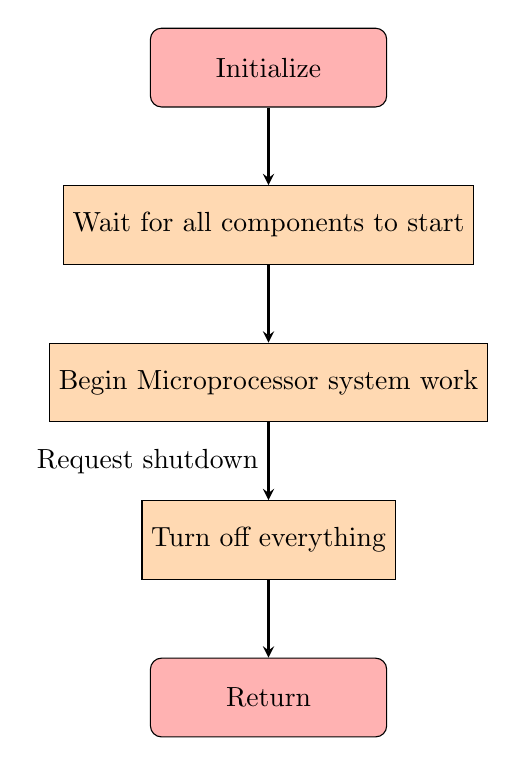
\begin{tikzpicture}[node distance=2cm]
        \node (start) [startstop] {Initialize};  
   	\node (wait) [process, below of = start] {Wait for all components to start};
	\node (main) [process, below of = wait] {Begin Microprocessor system work};
        \node (end) [process, below of = main] {Turn off everything};            
        \node (return) [startstop, below of = end] {Return};
	\draw [arrow] (start) -- (wait); 
	\draw [arrow] (wait) -- (main);
	\draw [arrow] (main) -- node[anchor=east] {Request shutdown} (end);
	\draw [arrow] (end) -- (return);
\end{tikzpicture}
\end{figure}

\begin{figure}[H]
	\caption{Main loop}
	\centering
	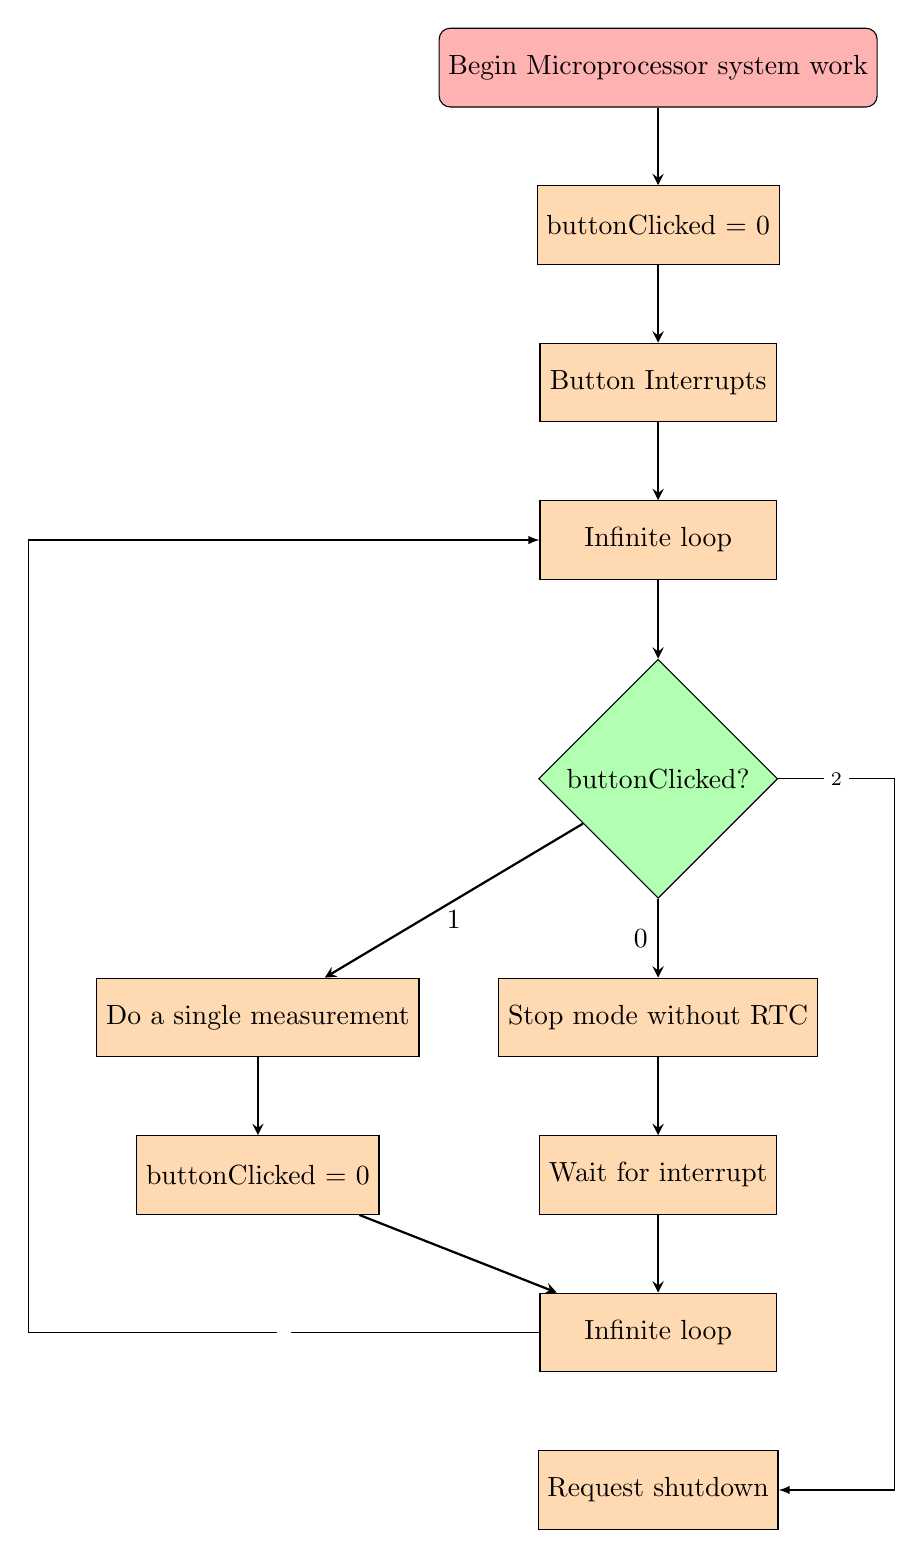
\begin{tikzpicture}[node distance=2cm]
		\node (beginMain) [startstop] {Begin Microprocessor system
			work};
		\node (setButtonClicked) [process, below of = beginMain]
			{buttonClicked = 0};
	\node (buttonInterrupts) [process, below of = setButtonClicked] {Button Interrupts};
	\node (infiniteLoop) [process, below of = buttonInterrupts] {Infinite
		loop};
	\node (whichButton) [decision, below = 1 cm of infiniteLoop] {buttonClicked?};
	\node(idle) [process, below = 1 cm of whichButton] {Stop mode without RTC};
	\node(freeze) [process, below of = idle] {Wait for interrupt};
	\node (infiniteLoop2) [process, below of = freeze] {Infinite loop};
	\node (endCompass) [process, below of = infiniteLoop2] {Request shutdown};
	\node(updateCompass) [process, left = 1 cm of idle] {Do a single
		measurement};
	\node(resetButton) [process, below of = updateCompass] {buttonClicked =
		0};
	\draw [arrow] (beginMain) -- (setButtonClicked);
	\draw [arrow] (setButtonClicked) -- (buttonInterrupts);
	\draw [arrow] (buttonInterrupts) -- (infiniteLoop);
	\draw [arrow] (infiniteLoop) -- (whichButton);
	\draw [arrow] (whichButton) -- node [anchor=east] {0} (idle);
	\draw [arrow] (whichButton) -- node [anchor=north] {1} (updateCompass);
	\draw [arrow] (updateCompass) -- (resetButton);
	\draw [arrow] (resetButton) -- (infiniteLoop2);
	\draw [arrow] (idle) -- (freeze);
	\draw [arrow] (freeze) -- (infiniteLoop2);
	\draw [rectangle connector=-8cm] (infiniteLoop2) to node[descr] {}  (infiniteLoop);
	\draw [rectangle connector=3cm] (whichButton) to node[descr] {2} (endCompass);
	\end{tikzpicture}
\end{figure}

\begin{figure}[H]
	\caption{Single measurement algorithm}
	\centering
	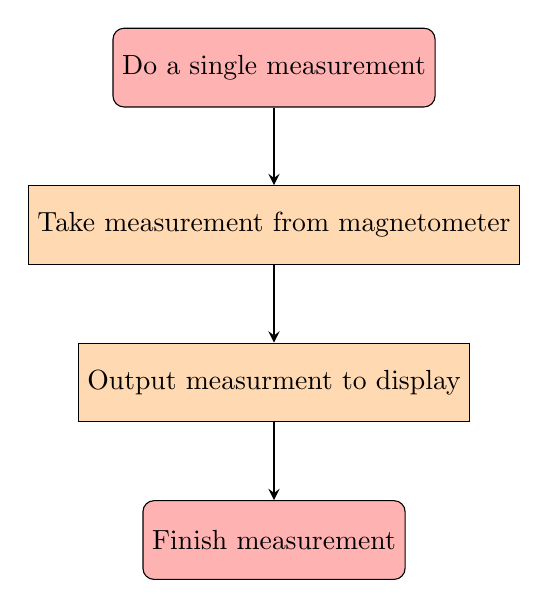
\begin{tikzpicture}[node distance = 2cm]
	\node (start) [startstop] {Do a single measurement};
		\node (askFor) [process, below of = start] {Take measurement
			from magnetometer};
		\node (process) [process, below of = askFor] {Output measurment
			to display};
		\node (end) [startstop, below of = process] {Finish
			measurement};
	\draw [arrow] (start) -- (askFor);
	\draw [arrow] (askFor) -- (process);
	\draw [arrow] (process) -- (end);
	\end{tikzpicture}
\end{figure}
\subsection{Description of the algorithm}
There are 3 main diagrams, start algorithm at the very beginning of the
microcontroller, then main loop containing most of the code and another one for
single measurement from magnetometer.
\begin{enumerate}
	\item Start algorithm - we initialize all of the components to be ready
		for the microcontroller to fork, we wait for the components to
		start and go into the main loop, once we get the shutdown
		interrupt we turn off all components and exit from the firmware.
	\item Main loop - Once all the components are initialized we start the
		main loop, we set the variable which tells us which button was
		clicked to default value of 0, we set up button interrupts to
		get information what button we clicked and we enter the infinite
		loop. In infinite loop depending on button clicked we either do
		a single measurement, shutdown the whole microprocessor or enter
		stop mode without RTC (lowest power consumption while still
		working with interrupts)
	\item Single measurement consists of taking data from magnetometer and
		outputing it on the display
\end{enumerate}
\begin{thebibliography}{9}
	\bibitem{datasheet} 
	\href{https://www.st.com/resource/en/datasheet/stm32l082cz.pdf}{STM32LO82CZ
	datasheet}
	\bibitem{consumerDevice}
	\href{https://www.st.com/en/microcontrollers-microprocessors/stm32l0-series.html}{Consumer
	Device STM32LOx2 Line}
	\bibitem{OLED}
	\href{https://www.mouser.pl/datasheet/2/291/NHD_2_7_12864WDY3-1116258.pdf}{OLED
	datasheet}
	\bibitem{Magnetometer}
	\href{https://cdn-shop.adafruit.com/datasheets/HMC5883L_3-Axis_Digital_Compass_IC.pdf}{Magnetometer
	datasheet}
	\bibitem{Battery}
	\href{https://www.murata.com/products/productdata/8809693839390/LR44R-DATASHEET.pdf?1604287808000}{Battery}
	\bibitem{Voltage Regulator}
	\href{https://www.analog.com/media/en/technical-documentation/data-sheets/3525fc.pdf}{Voltage
	regulator} 
\end{thebibliography}
\end{document}

